\subsection{Разработка алгоритма взаимодействия с программным средством}
\label{sec:design:app}

Далее рассматривается вопрос взаимодействия пользователя с программным средством.
Известно, что удобство пользования программным средством может во многом определять успешность проекта в целом~\cite[с.~44]{code_complete}.

Схема работы программного средства представлена на рисунке~\ref{fig:design:app:diagram}.
Среди ее особенностей можно выделить в высокой степени соответствие диаграмме прецедентов, которая была составлена и рассмотрена в пункте~\ref{sec:domain:use_cases}.

При входе в приложение пользователю должен предоставляться выбор списка сущностей, с которыми он может работать (также возможно отображение одного из списков по умолчанию с возможностью перехода к остальным).
Как видно из рисунка~\ref{fig:design:app:diagram}, за взаимодействие с пользователем отвечают три основных модуля: модуль работы с транзакциями, модуль работы со счетами и модуль работы с категориями.

Стоит отметить некоторые особенности приложения с точки зрения взаимодействия с пользователем:
\begin{itemize}
    \item основу проектируемого приложения предполагается расположить на трёх главных формах (экранах), каждая из которых отвечает за взаимодействие с конкретным логическим модулем;
    \item операции по созданию новых сущностей должны осуществляться через отдельные элементы управления, по модификации существующих данных -- через работу с элементами списков;
    \item сводные значения по счетам отображаются на той же форме, что и список счетов;
    \item после каждой операции с данными соответствующий список\linebreakобновляется;
    \item операция создания денежного перевода осуществляется через выбор счёта-отправителя из списка существующих счетов;
    \item при удалении категории требуется дополнительный выбор политики удаления зависимых транзакций.
\end{itemize}

Таким образом, составленная схема будет использована при разработке навигации по экранам программного средства.

\begin{figure}[p]
    \centering
    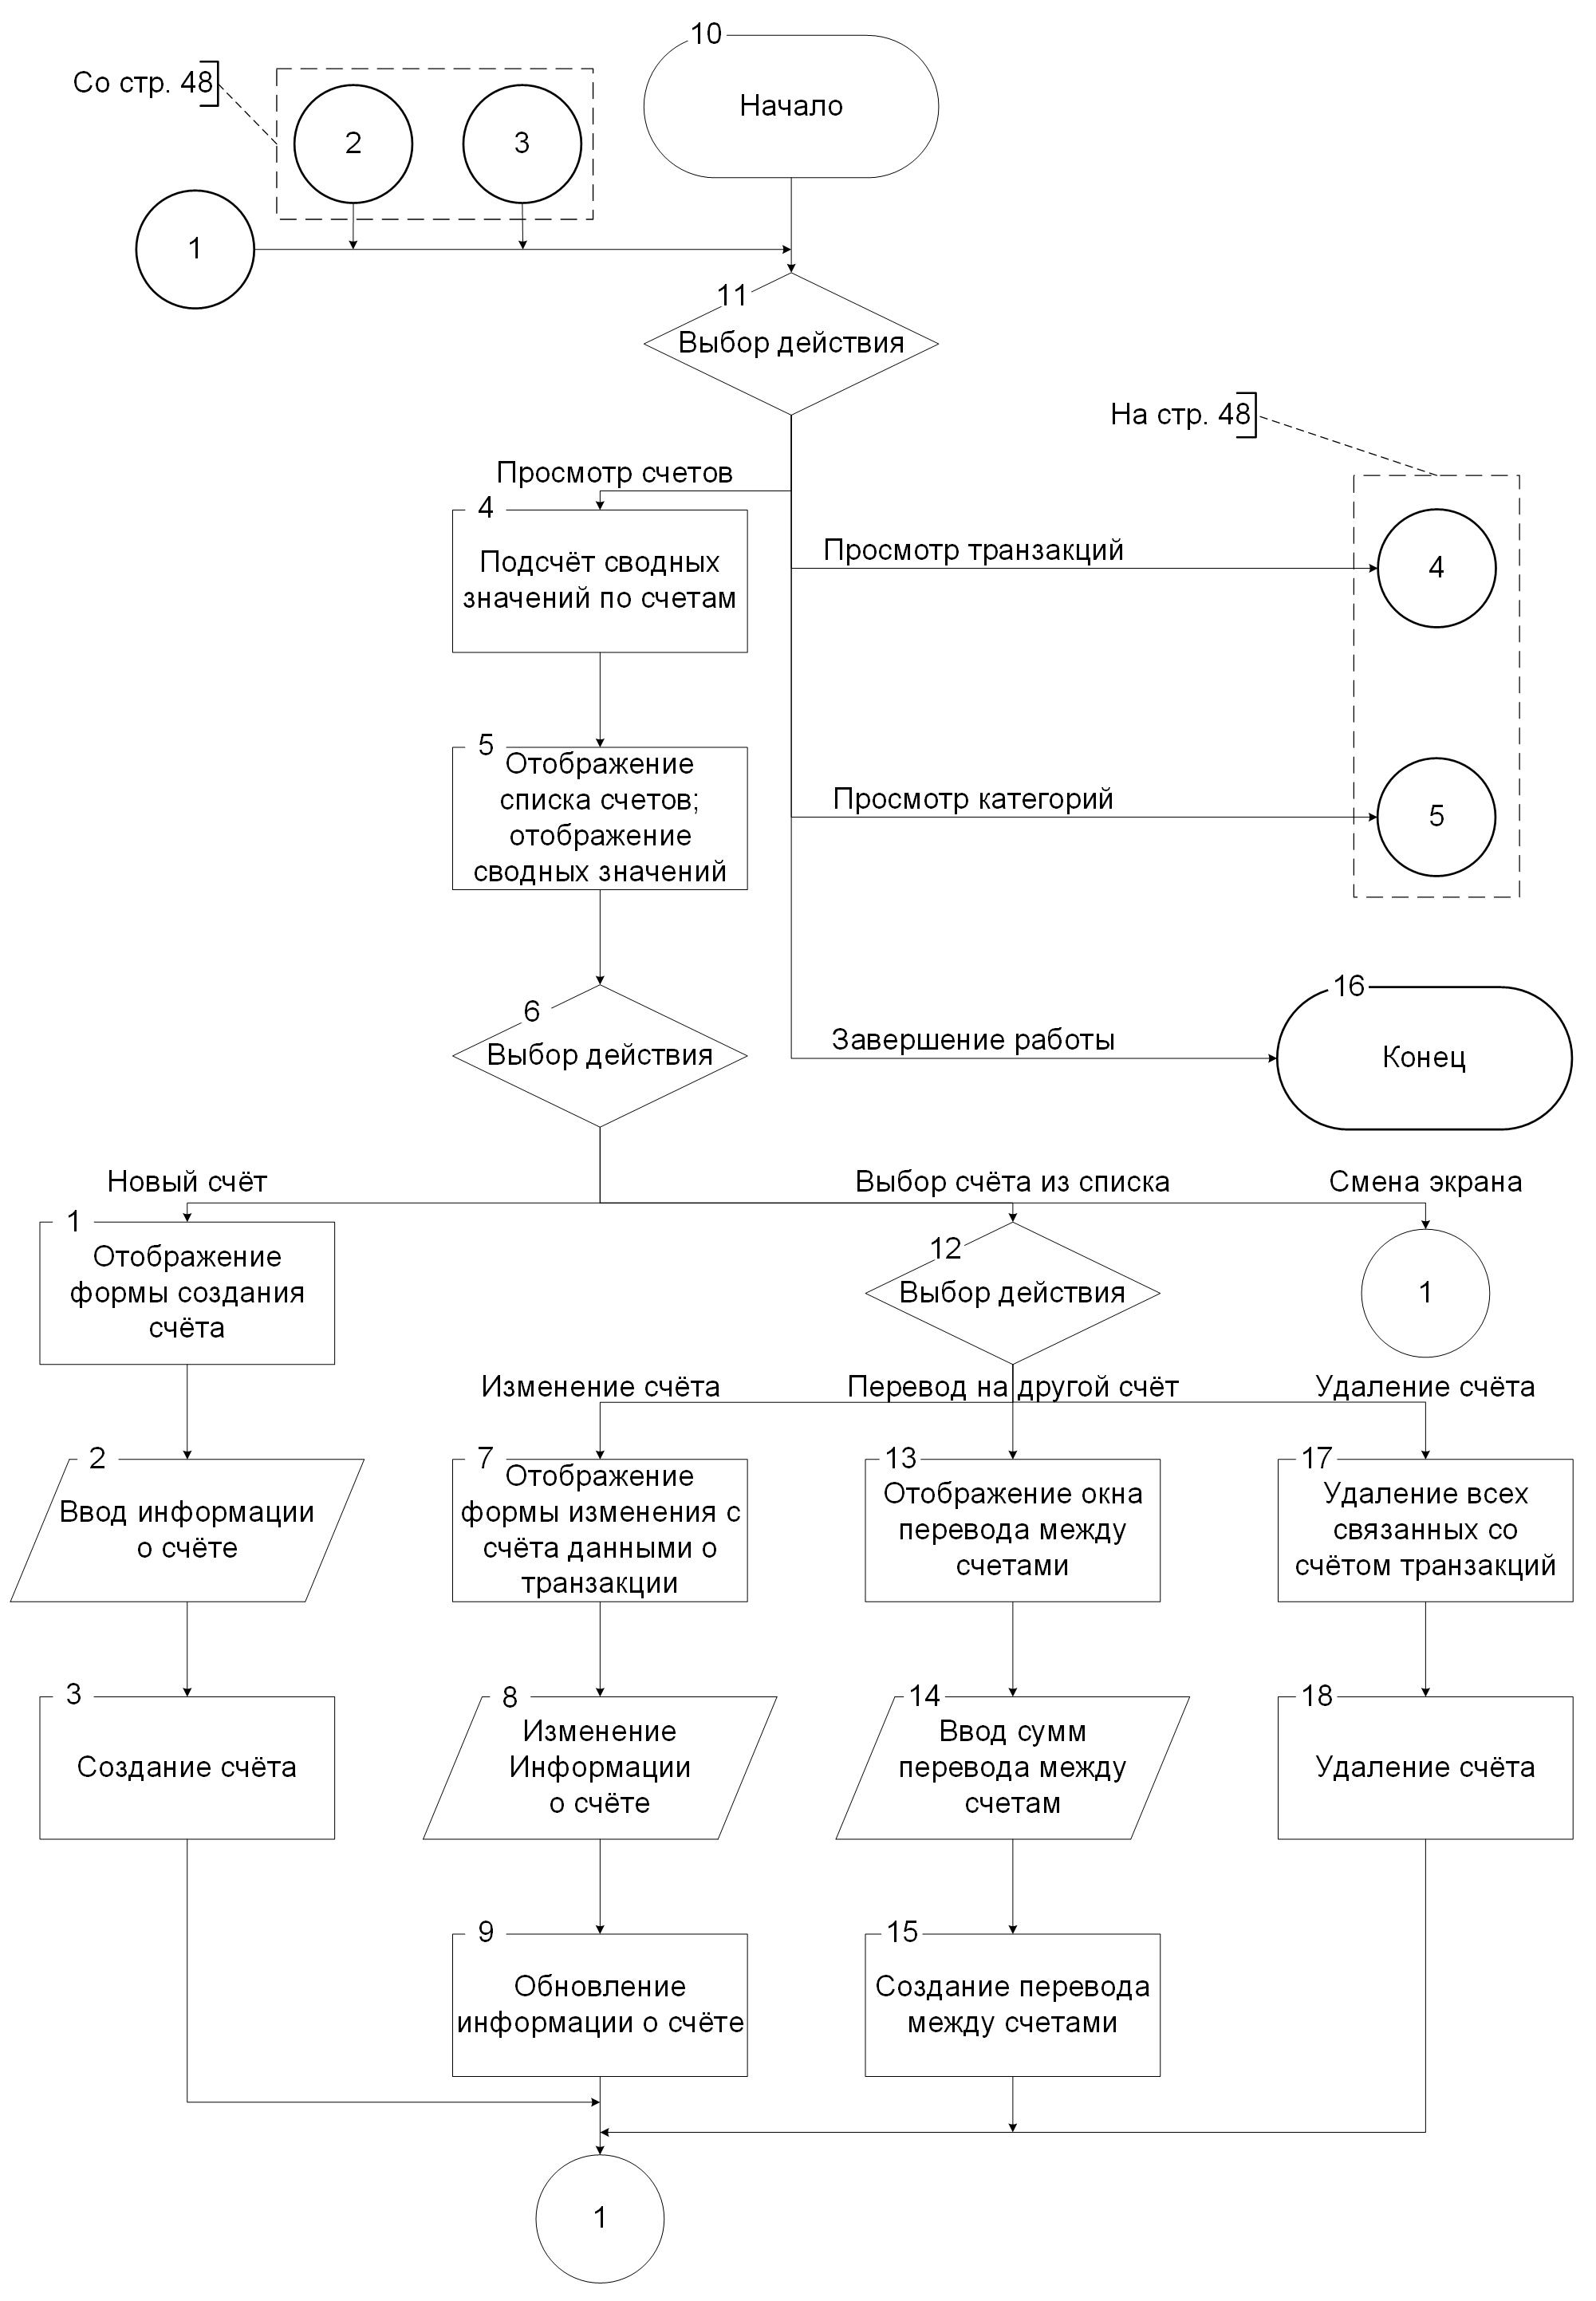
\includegraphics[scale=0.31]{3_5_app_diagram_1.png}
    \caption{Схема программы приложения}
    \label{fig:design:app:diagram}
\end{figure}

\begin{sidewaysfigure}
    \centering
    \ContinuedFloat
    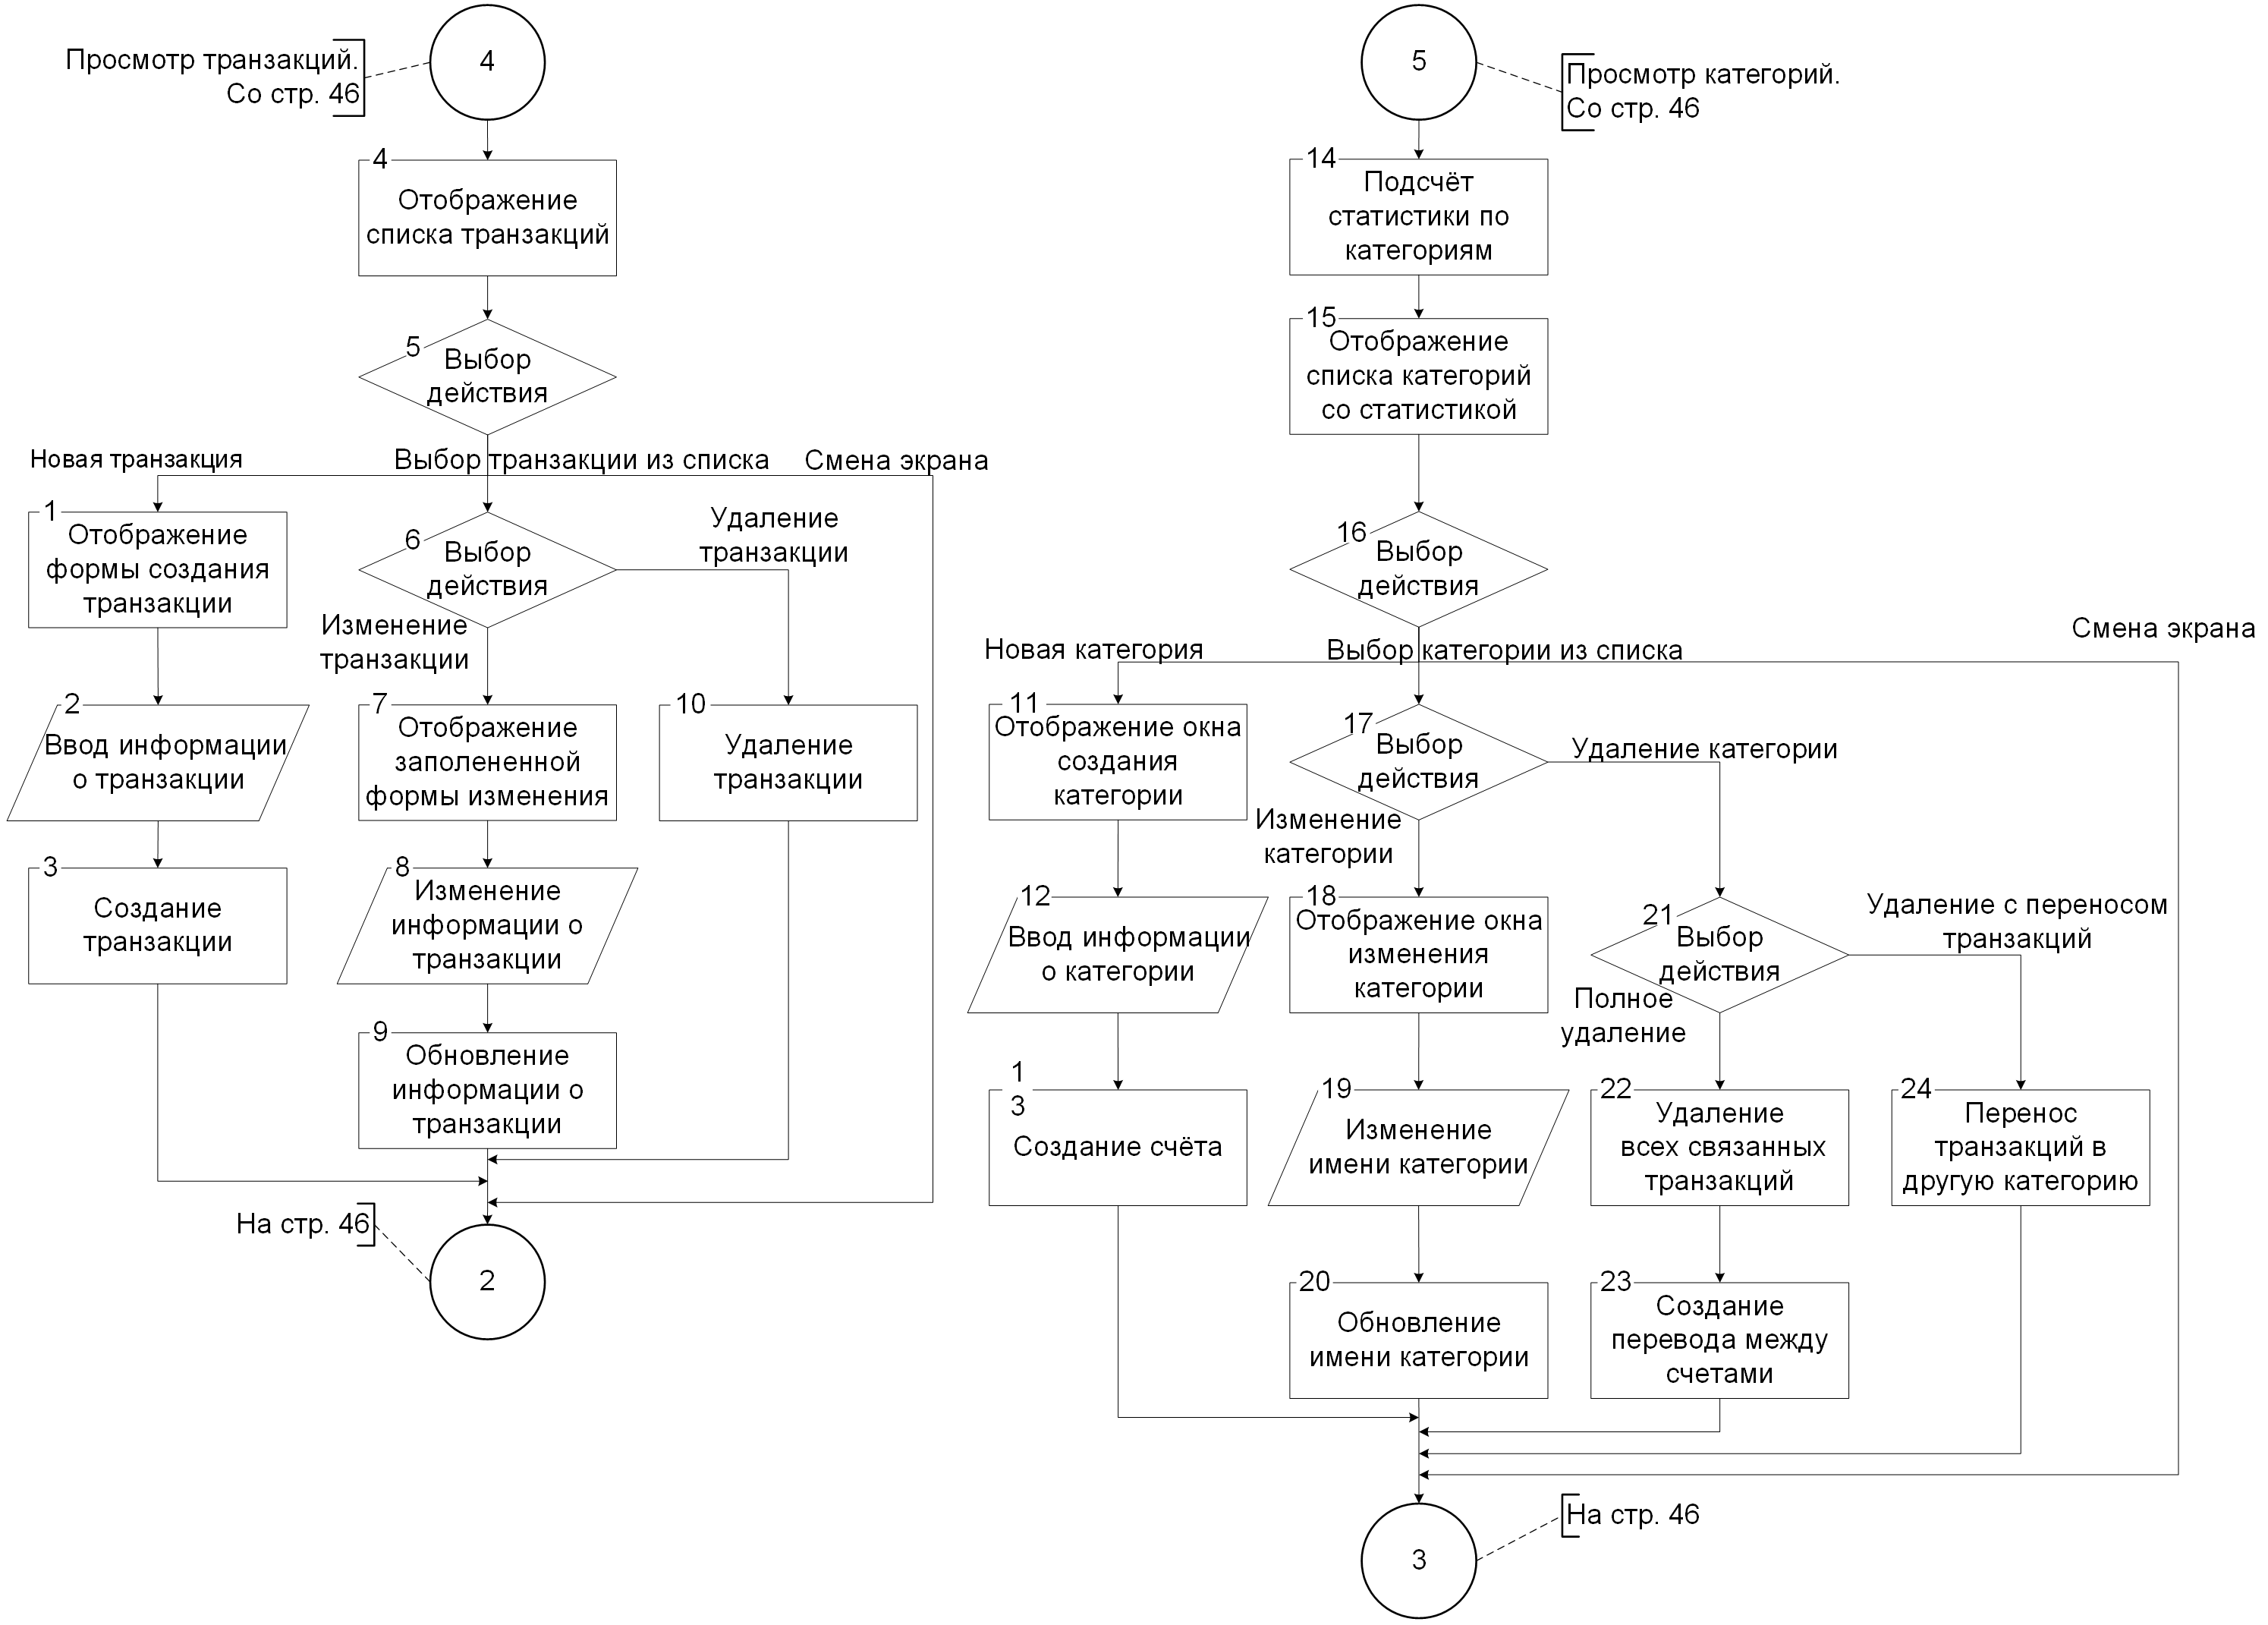
\includegraphics[scale=0.28]{3_5_app_diagram_2.png}
    \caption{Схема программы приложения (окончание)}
\end{sidewaysfigure}

